
\chapter{Constitutive theories}

The balance laws for mass, momentum, and energy and the imbalance law for entropy represent fundamental principles of continuum thermomechanics and as such are presumed to hold for all bodies, whether they be solid, liquid, or gas. In contrast, the constitution of a class of bodies composed of a particular material is specified by \textit{constitutive} equations. Such equations limit the class of ``processes'' that bodies comprised of a given material may undergo.

\section{Constitutive response functions and constitutive principles}
A constitutive equation gives the pointwise values of a physical field $\Phi$ in terms of the values of another such field (or list of such fields) $\Lambda$:
\begin{equation}
	\Phi(\xb,t)=\widehat{\Phi}(\Lambda(\xb,t),x).
\end{equation}
The function $\widehat{\Phi}$ is referred to as a \textit{constitutive response function}. We will skip the dependence on $\xb$, not presuming homogeneity.

In this section, we offer some general observations on the constitutive behavior of materials. These concepts will be examined in greater depth in the following chapters, focusing on specific classes of materials.

The primary fields considered in continuum mechanics include the velocity vector \( \mathbf{v}(\mathbf{y}, t) \), mass density \( \rho(\mathbf{y}, t) \), Cauchy stress tensor \( \mathbf{T}(\mathbf{y}, t) \), heat flux vector \( \mathbf{q}(\mathbf{y}, t) \), specific internal energy \( \varepsilon(\mathbf{y}, t) \), specific entropy \( \eta(\mathbf{y}, t) \), and temperature \( \vartheta(\mathbf{y}, t) \). These quantities are governed by the following balance laws and inequality:

\begin{definition}
	\begin{equation}\label{fieldeq}
	\begin{aligned}
		\dot{\rho} + \rho\, \text{div}\, \mathbf{v} &= 0, && \text{(Mass conservation)} \\
		\text{div}\, \mathbf{T} + \rho \mathbf{b} &= \mathbf{0}, && \text{(Force balance)} \\
		\mathbf{T} &= \mathbf{T}^\top, && \text{(Moment balance)} \\
		\mathbf{T} \cdot \mathbf{D} + \text{div}\, \mathbf{q} + \rho r &= \rho \dot{\varepsilon}, && \text{(Energy balance)} \\
		\rho \dot{\eta} &\geq \text{div} \left( \frac{\mathbf{q}}{\vartheta} \right) + \frac{\rho r}{\vartheta}, && \text{(Entropy inequality)}
	\end{aligned}
\end{equation}
\end{definition}

Here, \( \mathbf{b}(\mathbf{y}, t) \) is the body force per unit mass, and \( r(\mathbf{y}, t) \) represents the rate of heat supply per unit mass, both of which are considered to be given externally.

\vspace{1em}

These governing equations apply universally to any material, provided it is modeled as a continuum. Although everyday experience reveals that various materials exhibit different responses to identical external actions, such material-specific behavior is not captured at this stage of the theory.

%--------------------------------------------------------------------
%  Re-phrased discussion of constitutive relations
%--------------------------------------------------------------------

When the system \eqref{fieldeq} is written component-wise, and the Cauchy
stress is taken to be symmetric, one counts
\(16\) independent scalar fields ($\rho$, 3 for $\vb$, 6 for $\Tb$, 3 for $\qb$, $\varepsilon$, $\eta$, $\vartheta$) but only \(5\) genuine balance
equations—the entropy statement being an inequality.
Thus, \(11\) additional scalar relations are required to close the
system; these are supplied by the
\emph{constitutive equations} that describe the material response.

\vspace{0.5em}

\noindent
A material is therefore specified by a collection of response mappings
\[
\widehat{\mathbf{T}},\;
\widehat{\mathbf{q}},\;
\widehat{\varepsilon},\;
\widehat{\eta},
\]
whose task is to deliver, at the present instant, the values of
stress, heat flux, specific internal energy and specific entropy at
each material point, given the entire past history of the motion
\(\mathbf{y}(\mathbf{x},t)\) and of the temperature field
\(\vartheta(\mathbf{x},t)\).

\vspace{0.5em}

\noindent
A simple example (yet already non-trivial) set of constitutive
relations can be written as
\begin{equation}
		\begin{aligned}
			\mathbf{T} &= \widehat{\mathbf{T}}\bigl(\mathbf{F},\dot{\mathbf{F}},\vartheta\bigr),\\[2pt]
			\mathbf{q} &= \widehat{\mathbf{q}}\bigl(\mathbf{F},\vartheta,\grad\vartheta\bigr),\\[2pt]
			\varepsilon &= \widehat{\varepsilon}\bigl(\mathbf{F},\vartheta\bigr),\\[2pt]
			\eta &= \widehat{\eta}\bigl(\mathbf{F},\vartheta\bigr),
	\end{aligned}
\end{equation}
with \(\mathbf{F} = \nabla\mathbf{y}\) and
\(\dot{\mathbf{F}}\) its material time derivative.
Because \(\widehat{\mathbf{T}}\) is assumed symmetric, these relations
encode \(11\) scalar equations.

\vspace{0.5em}

\noindent
Determining the explicit form of the response mappings can rely on
\emph{ab initio} (atomistic) calculations, laboratory experiments, or
a suitable combination of the two.
A natural question is whether these mappings are completely free from
the standpoint of continuum theory, or whether the framework already
supplies internal restrictions that lessen the number of independent
functions one ultimately has to identify.
The remainder of this chapter addresses precisely that question, and
the discussion is organised around the following points:
\begin{enumerate}
	\item \textbf{Causality.}\;
	No present value of any field is allowed to depend on future
	values of that or any other field.
	\item \textbf{Field equations.}\;
	The moment balance enforces the symmetry of
	\(\widehat{\mathbf{T}}\).
	Body forces \(\mathbf{b}\) and volumetric heat supplies \(r\),
	being externally prescribed, may always be chosen
	\emph{a posteriori} so that the force and energy
	balances are met; hence those
	equations do not constrain the constitutive mappings.
	The only non-trivial restriction that remains stems from the
	entropy inequality.



Once the volumetric heat supply \(r\) has been selected so that the
energy balance \eqref{fieldeq}\(_4\) is satisfied, the entropy statement no longer
contains any quantities that may be chosen at will; it therefore becomes
an intrinsic constraint on the response of the material, through the reduced dissipation inequality
\begin{equation}
	\rho\,\dot{\psi}
	- \mathbf{T}\!\cdot\!\mathbf{D}
	+ \rho\eta\,\dot{\vartheta}
	- \frac{\mathbf{q}\!\cdot\!\operatorname{grad}\vartheta}{\vartheta}
	\;\le\; 0.
\end{equation}
%or, when written with respect to the reference configuration,
%\[
%\rho_{\rm ref}\,\dot{\psi}
%- \mathbf{S}\!:\!\dot{\mathbf{F}}
%+ \rho_{\rm ref}\eta\,\dot{\vartheta}
%- \frac{\mathbf{q}_{\rm ref}\!\cdot\!\nabla\vartheta}{\vartheta}
%\;\le\; 0.
%\]
Consequently, the entropy principle enforces specific restrictions on
the permissible constitutive mappings.



	\item \textbf{Material frame indifference.}\;
	The objectivity arguments of Chapter \ref{FI} clarify the
	transformation of physical fields between two motions that differ
	only by a rigid‐body displacement.  For instance,
	\(\varepsilon^{+}=\varepsilon\),
	\(\mathbf{F}^{+}= \mathbf{Q}\mathbf{F}\), and
	\(\vartheta^{+}=\vartheta\),
	where \(\mathbf{Q}\) is a proper orthogonal tensor.
	Suppose the energy response is given by
	\(\varepsilon = \widehat{\varepsilon}(\mathbf{F},\vartheta)\).
	In the transformed motion one obtains
	\(\varepsilon^{+} =
	\widehat{\varepsilon}(\mathbf{F}^{+},\vartheta^{+}) =
	\widehat{\varepsilon}(\mathbf{Q}\mathbf{F},\vartheta)\).
	Objectivity demands \(\varepsilon^{+}=\varepsilon\) for every
	\(\mathbf{Q}\in\mathrm{Rot}\), whence
	\[
	\widehat{\varepsilon}(\mathbf{F},\vartheta) =
	\widehat{\varepsilon}(\mathbf{Q}\mathbf{F},\vartheta)
	\quad
	\forall\,\mathbf{Q}\in\mathrm{Rot}.
	\]
	This requirement typifies the limitations that frame indifference
	imposes on the constitutive functions.
	
	\item \textbf{Material symmetry.}\;
	Whenever microstructural information reveals that the body enjoys
	specific symmetry operations—for example, a cubic lattice in a
	single crystal—those symmetries must be reflects at the continuum
	level.  Enforcing the same operations on the constitutive mappings
	reduces the number of independent material parameters and is an
	essential step in building realistic constitutive models.
\end{enumerate}

\begin{remark}
	For internal consistency, if we allow one of the constitutive response
	functions in the set $\widehat{\Tb}$, $\widehat{\qb}$, $\widehat{\varepsilon}$, $\widehat{\eta}$  to depend on a particular quantity, say temperature gradient,
	then we have no a priori reason not to allow all of them to depend on this quantity. Such a starting point is motivated by the belief that the underlying physics should determine which of the constitutive interactions are
	inappropriate, at least in a general theory. This, in essence, is Truesdell’s \textit{principle of equipresence}: ``A
	quantity present as an independent variable in one constitutive equation should be so present in all,
	unless\ldots its presence contradicts some law of physics or rule of invariance.''  Truesdell and Noll
	assert that: ``This principle forbids us to eliminate any of the `causes’ present from
	interacting with any other as regards a particular `effect.’ It reflects on the scale of gross phenomena the
	fact that all observed effects result from a common structure such as the motions of molecules.'' Physics,
	not caprice, should rule out interactions.
\end{remark}


%\section{Some Examples of Constitutive Response
%	Functions}
%The particular way in which a specific constitutive response function depends on the motion
%and temperature depends on the characteristics of the material being modeled. For example,
%consider the stress and how it may depend on the motion.
%What follow are merely examples of stress response functions having some relevant properties. 
%
%\vspace{.5cm}
%\begin{enumerate}
%	\item \textit{No memory. Short range forces.}\\
%	Suppose  that the stress at a particle $X$  at a time $t$
%	depends only on the motion of the particles in an infinitesimal neighborhood of $X$ at that time $t$. In this case we might expect $\widehat{\Tb}$ to be given by
%	\begin{equation}
%		\widehat{\Tb}\big(\Fb(\xb,t)\big).
%	\end{equation}
%\item \textit{Short memory. Short range forces.} \\
%Suppose that the stress at a particle $X$ at a time $t$
%depends only on the motion of the particles in an infinitesimal neighborhood of $X$ at times
%up to and close to times preceding time $t$. Such a material has some slight memory of the
%past. In this case we might expect $\widehat{\Tb}$  to depend on $\Fb(\xb, t)$ as well some number of time
%derivatives of $\Fb$:
%\begin{equation}
%	\widehat{\Tb}\Big(\Fb(\xb, t), \dot\Fb(\xb, t),\ddot\Fb(\xb, t),\ldots \overset{(n)}{\Fb}(\xb,t)   \Big)
%\end{equation}
%\item \textit{Long memory. Short range forces.} \\
%Suppose that the stress at a particle $X$ at a time
%$t$ depends only on the motion of the particles in an infinitesimal neighborhood of $X$ at all
%times up to and preceding time $t$. Such a material has memory of the past. In this case we
%might expect  $\widehat{\Tb}$ to involve terms such as
%\begin{equation}
%	\int_{-\infty}^t e^{-(t-\tau)/\lambda}\fb\Big(\Fb(\xb,\tau)\,d\tau  \Big), \quad \lambda>0.
%\end{equation}
%\item \textit{No memory. Medium range forces.} \\
%Suppose that the stress at a particle $X$ at a time
%$t$ depends only on the motion of the particles in a small but not infinitesimal neighborhood
%of $X$ at that time $t$. Such a material is said to be \textit{nonlocal}. In this case we might expect $\widehat{\Tb}$
%to depend on $\Fb(\xb, t)$ as well as some spatial derivatives of F:
%\begin{equation}
%\widehat{\Tb}=\Big( \Fb(\xb, t), \nabla \Fb(\xb, t), \nabla\nabla \Fb(\xb, t) \Big).
%\end{equation}
%\item \textit{No memory. Long range forces.}\\
%Suppose that the stress at a particle $X$ at a time $t$
%depends only on the motion of all of the the particles of the body at that time $t$. In this case
%we might expect  $\widehat{\Tb}$ to involve terms such as
%\begin{equation}
%	\int_{\widetilde\Omega}e^{-\alpha|\xb-\xib|}\fb\Big(\fb(\xib-\xb,t)\Big)\,d\xib.
%\end{equation}
%\end{enumerate}
%The preceding are meant only to be illustrative and not exhaustive in any sense. There
%are other constitutive relations whose primitive form is quite different to the preceding.
\section{Examples of Constitutive Response Functions}

The specific form of a constitutive response function, and its dependence on motion and temperature, is determined by the nature of the material being modeled. For illustration, we focus here on how the stress may depend on the motion. The examples below are representative of stress response functions exhibiting various physically relevant features.

\vspace{0.5cm}

\begin{enumerate}
	\item \textit{No memory. Short-range forces.} \\
	Suppose that the stress at a material point $X$ and time $t$ depends only on the motion of particles in an infinitesimal neighborhood of $X$ at the same time $t$. In this case, we may expect the constitutive function $\widehat{\Tb}$ to have the form:
	\begin{equation}
		\widehat{\Tb} = \widehat{\Tb}\big(\Fb(\xb, t)\big).
	\end{equation}
	
	\item \textit{Short memory. Short-range forces.} \\
	Suppose that the stress at a material point $X$ and time $t$ depends on the motion of nearby particles not only at time $t$, but also at times slightly prior to $t$. The material exhibits a mild memory effect. In such a case, $\widehat{\Tb}$ may depend on the deformation gradient and its time derivatives:
	\begin{equation}
		\widehat{\Tb} = \widehat{\Tb}\Big(\Fb(\xb, t), \dot{\Fb}(\xb, t), \ddot{\Fb}(\xb, t), \ldots, \overset{(n)}{\Fb}(\xb, t)\Big).
	\end{equation}
	
	\item \textit{Long memory. Short-range forces.} \\
	Suppose that the stress at point $X$ and time $t$ depends on the entire past history of the motion in an infinitesimal neighborhood of $X$. Such a material possesses long-term memory. A typical form for $\widehat{\Tb}$ in this case may involve an integral over past times:
	\begin{equation}
		\widehat{\Tb} = \int_{-\infty}^t e^{-(t - \tau)/\lambda} \, \fb\big(\Fb(\xb, \tau)\big) \, d\tau, \quad \lambda > 0.
	\end{equation}
In this expression $e^{-(t - \tau)/\lambda}$ is  an exponential kernel that gives more weight to recent deformations (\textit{i.e.}, as $\tau\to t$) and less weight to remote past ($\tau\ll t$);
$\lambda>0$ is a relaxation time: for small $\lambda$ the material ``forgets'' quickly (short memory), for large $\lambda$ memory fades slowly.
An example of this class is visco-elasticity.

	
	\item \textit{No memory. Medium-range forces.} \\
	Suppose that the stress at point $X$ and time $t$ depends on the motion within a finite, but not infinitesimal, neighborhood of $X$ at that same time. Such materials are called \textit{nonlocal}. In this case, $\widehat{\Tb}$ may depend on spatial gradients of the deformation:
	\begin{equation}
		\widehat{\Tb} = \widehat{\Tb}\Big(\Fb(\xb, t), \nabla \Fb(\xb, t), \nabla\nabla \Fb(\xb, t)\Big).
	\end{equation}
	
	\item \textit{No memory. Long-range forces.} \\
	Suppose that the stress at point $X$ and time $t$ depends on the motion of all particles in the body at that same time. This global interaction can be expressed through a nonlocal integral over the entire body:
	\begin{equation}
		\widehat{\Tb} = \int_{\widetilde{\Omega}} e^{-\alpha |\xb - \xib|} \, \fb\big(\Fb(\xib - \xb, t)\big) \, d\xib.
	\end{equation}
Here $e^{-\alpha |\xb - \xib|} $ is  a weighting kernel that decays exponentially with distance. The parameter $\alpha>0$ controls how fast the influence of distant points decays: with large $\alpha$ there is a rapid decay, which turns out in a  nearly local behavior.
Possible applications are \textit{peridynamic} theory and \textit{nonlocal elasticity} models for nano-structured materials.
\end{enumerate}

These examples are intended to be illustrative rather than exhaustive. Many other types of constitutive relations exist, with forms that differ significantly from those presented here.


\section{A simple illustrative example}

In this section we present an elementary model to show how the twin
requirements of \emph{material frame indifference} and the
\emph{entropy inequality} constrain the admissible form of constitutive
laws.  As we shall see, these constraints can drastically simplify the
structure of the response functions.

%--------------------------------------------------------------------
%  1. Kinematics and balance laws
%--------------------------------------------------------------------
\subsection{Kinematics and field equations}

We restrict attention to the \emph{purely mechanical} description of a
continuum, involving only the motion
\(\mathbf{y}(\mathbf{x},t)\), the velocity
\(\mathbf{v}(\mathbf{y},t)\), the current mass density
\(\rho(\mathbf{y},t)\), the Cauchy stress
\(\mathbf{T}(\mathbf{y},t)\) and the Helmholtz free energy
\(\psi(\mathbf{y},t)\).
The kinematic relations are
\begin{equation}
	\mathbf{F} = \nabla\mathbf{y}, 
	\quad 
	J = \det\mathbf{F}, 
	\quad 
	\mathbf{v} = \dot{\mathbf{y}}, 
	\quad
	\mathbf{D} = \tfrac12\bigl(\mathbf{L}+\mathbf{L}^{\!\top}\bigr), 
	\quad 
	\mathbf{L} = \grad\mathbf{v},
\end{equation}
and the pertinent field equations read
\begin{equation}\label{ex}
		\begin{aligned}
			\dot\rho+\rho\dive\vb &=0, & & \text{(mass conservation)}, \\[2pt]
		%	\rho_{\rm ref} &= \rho J, & & \text{(mass conservation)}, \\[2pt]
			\dive\mathbf{T} + \mathbf{b} &= \mathbf{0}, & & \text{(force balance)}, \\[2pt]
			\mathbf{T} &= \mathbf{T}^{\!\top}, & & \text{(moment balance)}, \\[2pt]
			\mathbf{T}\cdot\mathbf{D} &\ge \rho\dot{\psi}, & & \text{(entropy inequality)}.
	\end{aligned}
\end{equation}
Equation \eqref{ex}\(_3\) is the purely mechanical counterpart of the
general dissipation inequality.


\subsection{Constitutive equations}

The fields \(\rho\), \(\psi\), \(\mathbf{y}\) and the symmetric tensor
\(\mathbf{T}\) comprise \(11\) scalar unknowns, whereas~\eqref{ex} offers
only \(4\) scalar equations; \(7\) additional relations are therefore
required.  As a working proposal, let the stress and free energy depend
on the motion only through the Jacobian,
\[
\mathbf{T} = \overline{\Tb}(J),
\qquad
\psi      = \overline{\psi}(J),
\qquad
J = \det\mathbf{F}.
\]
Because the mass balance links \(J\) and \(\rho\) via
\(\rho_{\rm ref} = \rho J\), an equivalent set is
\begin{equation}\label{conex}
	\mathbf{T} = \widehat{\mathbf{T}}(\rho),
	\qquad
	\psi      = \widehat{\psi}(\rho).
\end{equation}

The aim of this section is to show how objectivity and the entropy inequality impose
certain restrictions on the constitutive response function $\widehat{\Tb}$ and $\widehat{\psi}$. We shall start with the
set of constitutive relations \eqref{conex} that involve seven independent scalar constitutive functions; after ensuring that \eqref{conex}  is consistent with the requirements of objectivity and the entropy inequality, we will find that, in fact, they only involve \textit{one} independent scalar-valued
constitutive function.


\subsection{Restrictions due to objectivity}

Consider two motions that differ only by a
\emph{time‐dependent rigid rotation}:
\(\mathbf{y}^{+}(\mathbf{x},t) = \mathbf{Q}(t)\,\mathbf{y}(\mathbf{x},t)\)
with \(\mathbf{Q}\!\in\!\Rot\).
Since \(\det\mathbf{Q}=1\),
\[
J^{+} = \det(\mathbf{Q}\mathbf{F}) = J
\quad\Longrightarrow\quad
\rho^{+} = \rho
\quad\text{by \eqref{ex}\(_1\).}
\]
The constitutive proposal~\eqref{conex} yields
\begin{equation}
	\psi      = \widehat{\psi}(\rho), 
	\;\;
	\psi^{+}= \widehat{\psi}(\rho^{+}), 
	\qquad
	\mathbf{T}= \widehat{\mathbf{T}}(\rho), 
	\;\;
	\mathbf{T}^{+}= \widehat{\mathbf{T}}(\rho^{+}).
\end{equation}
As we stated, the frame indifference principle requires that the free energy be
rotation‐invariant and that the stress transform as 
\begin{equation}\label{frin}
	\psi^{+} = \psi,
	\qquad
	\mathbf{T}^{+} = \mathbf{Q}\,\mathbf{T}\,\mathbf{Q}^{\!\top}
	\quad
	\forall\;\mathbf{Q}\in\Rot.
\end{equation}




%\subsection{Restrictions implied by objectivity}

The first condition in~\eqref{frin} is automatically satisfied because
\(\rho^{+}=\rho\).
The second condition, combined with~\eqref{conex}, demands
\begin{equation}
	\widehat{\mathbf{T}}(\rho) =
	\mathbf{Q}\,\widehat{\mathbf{T}}(\rho)\,\mathbf{Q}^{\!\top}
	\quad
	\forall\;\rho>0,\ 
	\forall\;\mathbf{Q}\in\Rot.
\end{equation}
This equation forces \(\widehat{\mathbf{T}}\) to be
\emph{isotropic}, whence
\begin{equation}
\widehat{\mathbf{T}}(\rho)=-\widehat{p}(\rho)\,\mathbf{I}, \qquad \psi=\widehat{\psi}(\rho).
\end{equation}
where  \(\widehat{p}(\rho)\) is an arbitrary scalar-valued constitutive function, there being no restrictions on $\widehat{\psi}$. Notice that the 7 scalar constitutive functions
$\widehat{\Tb}$ and $\widehat{\psi}$ have been reduced by the requirement of objectivity to 2 independent scalar-valued constitutive functions  \(\widehat{p}(\rho)\) and $\widehat{\psi}(\rho)$.


\subsection{Restrictions due to entropy inequality}
We  now consider the entropy inequality \eqref{ex}$_4$. First notice that
\begin{equation}
\Tb\cdot\Db =-\widehat{p}(\rho)\Ib\cdot\Db=-\widehat{p}(\rho)\, \operatorname{tr}\Db=-\widehat{p}(\rho)\,\dive \vb=\widehat{p}(\rho)\frac{\dot\rho}{\rho},
\end{equation}
where we have used the mass balance $\dot{\rho}+\rho\dive\vb=0$. Therefore, the entropy inequality reads
\begin{equation}
\widehat{p}(\rho)\frac{\dot\rho}{\rho}\ge \rho \widehat{\psi}'(\rho)\,\dot\rho.
\end{equation}
This must hold in all thermodynamic process, posing therefore a restriction on the constitutive functions $\widehat{p}$ and $\widehat{\psi}$. Let us write the entropy inequality as
\begin{equation}\label{CNex}
\Big( -\widehat{p}(\rho)+\rho^2 \widehat{\psi}'(\rho) \Big)\, \dot{\rho}\leq0,
\end{equation}
and note that, since it must hold in all thermodynamic process, it must hold for all $\rho>0$ and all $\dot\rho$.  It follows that the term
in the parenthesis must vanish, since if it was either positive or negative, we could chose $\dot{\rho}$
to be negative or positive respectively, thus violating the inequality. Consequently we
find that the two constitutive functions $\widehat{p}$ and $\widehat{\psi}$ are not independent but are in fact related
\begin{equation}
\widehat{p}(\rho)=\rho^2\, \widehat{\psi}'(\rho).
\end{equation}

We then conclude that if a material is described by a set of constitutive equations of the form \eqref{conex}, in view of objectivity and the entropy inequality the must be of the form
\begin{equation}
\Tb=-\rho^2 \widehat{\psi}'(\rho), \qquad \psi=\widehat{\psi}(\rho).
\end{equation}

We notice that the 7 scalar constitutive equations we started with have been reduced to one independent scalar function $\widehat{\psi}$.

\begin{remark}
As previously stated, equation~\eqref{CNex} must be satisfied for every $\rho > 0$ and every $\dot{\rho}$. From this, we inferred that  
at any given spatial and temporal point $(\yb^\ast, t^\ast)$, the values of $\rho$ and $\dot{\rho}$ may be prescribed  
independently and without constraint. To illustrate this, consider a uniform velocity field defined by $\vb(\yb, t) = \Lb \yb$,  
with $\Lb$ an arbitrary constant tensor. Define $\beta = \operatorname{tr} \bm{L} = \operatorname{div} \vb$, which is also constant.  

Let us consider a spatially uniform mass density field $\rho(t)>0$, satisfying  $\rho(t^\ast)=\alpha$, for some time $t^\ast$ and arbitrary constant $\alpha$. Now, in order to satisfy the mass balance,  $\dot{\rho} + \rho \,\beta = 0$, which yields
\[
\rho(t) = \alpha e^{-\beta(t - t^\ast)}
\]  
where $\alpha > 0$ is an arbitrary constant. It is straightforward to verify that $\rho(t)$ remains positive for all times $t$.  
We therefore have that  $\rho(t^\ast) = \alpha$ and $\dot{\rho}(t^\ast) = -\alpha \beta$.  
Since both $\alpha > 0$ and $\beta$ can be freely and independently chosen,  
this confirms that $\rho(t^\ast)$ and $\dot{\rho}(t^\ast)$ can likewise be independently specified,  
as originally asserted.


\end{remark}

%\subsection{Frame-indifference and compatibility with thermodynamics}
%We  require that \textit{constitutive equations 
%	\begin{itemize}
%		\item be invariant under changes of frame,
%		\item be compatible with thermodynamics.
%\end{itemize}}
%The first hypothesis is the referred to as \textit{frame-indifference}. More specifically this means that
%\begin{equation}
%	\textrm{if} \quad \Phi=\widehat{\Phi}(\Lambda) \quad \textrm{then} \quad \Phi^+=\widehat{\Phi}(\Lambda^+) .
%\end{equation}
%
%To satisfy the second hypothesis, we utilize a procedure invented by Coleman \& Noll in 1964, a procedure under which only constitutive equations that are consistent with the free-energy inequality in all processes are deemed physically viable.  
%
%We exemplify both the requirements in the context of continuum thermomechanics. To begin with, rigid conductors will be faced, where  invariance has not in fact role, but Coleman \& Noll procedure may be easier clarified.
%
%
%The reduced dissipation inequality \eqref{DDR} limits the class of possible processes. To understand its role, in this chapter, we will analyze, within the context of three-dimensional continuum mechanics, some classes of materials:
%\begin{enumerate}
%	\item \textit{Elastic materials}, thermal insulators;%, for which the list of state variables is $\Sc=\{\Eb\}$ and for which $\qb =\mathbf{0}$ and $\dot{\vartheta}=0$;
%	\item \textit{Rigid conductors};%, for which $\Eb=\mathbf{0}$ and for which $\Sc=\{  \vartheta, \nabla\vartheta\}$;
%	\item \textit{Elastic conductors}.%, for which $\Sc=\{ \Eb, \vartheta, \nabla\vartheta\}$.
%\end{enumerate}














\chapter{Elastic Materials}
An elastic material has no memory of its past. Moreover, the response at a particle $\xb$ depends only on the motion of the particles in an infinitesimal neighborhood of it. Thus as
far as dependency on the motion goes, the constitutive response functions depend on the
motion solely through the current value of the deformation gradient tensor at $\xb$: $\Fb(\xb, t)$.
%Moreover, an elastic material does not dissipate energy:
%	\begin{equation}\label{gammael}
%	\rho\gamma = \Tb \cdot \Db - \rho\dot{\psi} = 0.
%\end{equation}

An elastic material is characterized by a set of constitutive relations
\begin{equation}
	\Tb=\widehat{\Tb}(\Fb), \qquad \varepsilon=\widehat{\varepsilon}(\Fb),
\end{equation}
or equivalently
\begin{equation}
	\Pb=\widehat{\Pb}(\Fb), \qquad \psi=\widehat{\psi}(\Fb).
\end{equation}
The constitutive response functions for stress are assumed to satisfy the moment balance requirements
\begin{equation}
\widehat{\Tb}(\Fb)=\widehat{\Tb}^\top(\Fb), \qquad \widehat{\Pb}(\Fb)\Fb^\top=\Fb\widehat{\Pb}(\Fb),
\end{equation}
for all nonsingular $\Fb$.

\section{Implications of the Entropy Inequality}
The  argument used to determine the consequences of the entropy inequality i known as the \textit{Coleman-Noll Procedure}.\footnote{See B.D. Coleman, W. Noll, The thermodynamics of elastic materials with heat conduction and viscosity, Arch. Rational Mech. Anal., 13 (1963), pp. 167-178.}
It is convenient for our present purposes to consider the referential constitutive characterization. Let us consider the reduced dissipation inequality  written in  a purely mechanical context:
\begin{equation}
\rho_{0} \dot\psi-\Pb\cdot\dot\Fb\leq0,
\end{equation}
where $\rho_{0}$ is the referential mass density. Substituting the constitutive maps, we get
\begin{equation}
	\Big(\rho_{0} \partial_\Fb\widehat{\psi}(\Fb)-\widehat{\Pb}(\Fb)\Big)\cdot\dot\Fb\leq0.
\end{equation}
The fact that this inequality must hold in all dynamical processes implies that it must hold for all arbitrarily chosen tensors $\dot\Fb$. It follows that 
\begin{definition}
	\begin{equation}
\widehat{\Pb}(\Fb)=\rho_{0} \partial_\Fb\widehat{\psi}(\Fb).
\end{equation}
\end{definition}

Observe that in order to characterize an elastic material it is only necessary to
specify the  constitutive response function $\widehat{\psi}(\Fb)$.

\section{Implications of Material Frame Indifference}
We now explore the implications of material frame indifference on the constitutive response
function $\widehat{\psi}(\Fb)$. Throughout this discussion we will be concerned with two processes $\yb^+$ and $\yb$, which are related to each other by
\begin{equation}
\yb^+(\xb,t)=\Qb(t)\yb(\xb,t),
\end{equation}
where $\Qb(t)$ is a rotation tensor at each time.

Let $\Fb^+$, $\psi^+$ and $\Fb$, $\psi$ the deformation gradient tensors and the Helmholtz free-energy in these two processes.  Then the constitutive
relation, when applied to these two processes, yield
\begin{equation}
\psi=\widehat{\psi}(\Fb), \qquad \psi^+=\widehat{\psi}(\Fb^+).
\end{equation}
From our previous discussion on objectivity, we know that
\begin{equation}
\Fb^+=\Qb\Fb, \qquad \psi^+=\psi.
\end{equation}
Constitutive laws should be independent of the observer and therefore
\begin{equation}\label{psiq}
\widehat{\psi}(\Qb\Fb)=\widehat{\psi}(\Fb)
\end{equation}
for all tensors $\Fb$ with positive determinant, all proper orthogonal tensors $\Qb$. Equation \eqref{psiq} places restrictions on the constitutive response $\widehat{\psi}$. For example
the function $\widehat{\psi}(\Fb)=\operatorname{tr}\Fb^\top\Fb$ does satisfy  \eqref{psiq} , but $\widehat{\psi}(\Fb)=\operatorname{tr}\Fb$ does not.

Next we turn our attention to determining the most general constitutive response function  $\widehat{\psi}(\Fb)$ which are consistent with  \eqref{psiq}.  We begin by deriving a necessary condition implied by equation~ \eqref{psiq} . Since  \eqref{psiq}  is to hold for all  
rotations \( \mathbf{Q} \), it must in particular hold for the specific choice \( \mathbf{Q} = \mathbf{R}^\top \),  
where \( \mathbf{R} \) is the rotational part in the polar decomposition \( \mathbf{F} = \mathbf{R} \mathbf{U} \).  
Then, equation~ \eqref{psiq} implies  

\begin{definition}
	\begin{equation}\label{psiU}
	\widehat{\psi}(\mathbf{F}) = \widehat{\psi}(\mathbf{U}) 
\end{equation}
\end{definition}

where \( \mathbf{U} = \sqrt{\mathbf{F}^\top \mathbf{F}} \) is the right stretch tensor.  


Conversely, let \( \widehat{\psi}(\cdot) \) be any real-valued function defined for tensors with positive determinant  
that satisfies equation~\eqref{psiU}. Then, since \( \mathbf{Q} \mathbf{F} = \mathbf{Q} (\mathbf{R} \mathbf{U}) = (\mathbf{Q} \mathbf{R}) \mathbf{U} \),  
the rotational and right stretch factors in the (unique) polar decomposition of \( \mathbf{Q} \mathbf{F} \) are \( \mathbf{Q} \mathbf{R} \) and \( \mathbf{U} \), respectively.  
Thus, when equation~\eqref{psiU} holds, it follows that  
\[
\widehat{\psi}(\mathbf{Q} \mathbf{F}) = \widehat{\psi}(\mathbf{U})
\]  
for all \( \mathbf{F} \) with positive determinant and all rotations \( \mathbf{Q} \), where \( \mathbf{U} = \sqrt{\mathbf{F}^\top \mathbf{F}} \).  
We conclude that equation~ \eqref{psiq} holds.  
Therefore, condition~\eqref{psiU} both necessary and sufficient for equation~ \eqref{psiq}  to be satisfied.


\begin{remark}
	Intuitively, we would have expected the free energy to not depend on the rotation,
	and therefore that it should depend on $\Fb$ only through the stretch. However it may not have
	been immediately obvious as to which of the two stretches $\Ub$ and $\Vb$ would be appropriate.
	The above analysis shows that it is $\Ub$. Intuitively, we could have guessed this too, since
	frame indifference states that a post-rotation doesn't affect the energy; it does not refer to a
	prerotation (which as we shall discuss later is related to the symmetry of the material, and
	which would, in general, affect the energy).
\end{remark}

We conclude that the most general set of constitutive response functions for an elastic material
that is both frame-indifferent and consistent with the second law of thermodynamics is
\begin{equation}
	\psi=\widehat{\psi}(\Ub).
\end{equation}
Since $\Cb=\Ub^2$, we can define $\widetilde{\psi}$ by  $\widetilde{\psi}(\Cb)=\widehat{\psi}(\sqrt{\Cb})$, and therefore
\begin{equation}
	\widehat{\Pb}=\rho_0\partial_\Fb \widetilde{\psi}(\Cb).
\end{equation}
This relation can be written as
\begin{equation}
P_{ij}=\rho_0\frac{\partial \widetilde{\psi}}{\partial F_{ij}}=\rho_0\frac{\partial \widetilde{\psi}}{\partial C_{hk}}\frac{\partial C_{hk}}{\partial F_{ij}}.
\end{equation}
Now
\begin{equation}
	C_{hk}=(\Fb^\top)_{hl}F_{lk}=F_{lh}F_{lk},
\end{equation}
and then
\begin{equation}
\frac{\partial C_{hk}}{\partial F_{ij}}=\frac{\partial F_{lh}}{\partial F_{ij}}F_{lk}+F_{lh}\frac{\partial F_{lk}}{\partial F_{ij}}=\delta_{li}\delta_{hj}F_{lk}+\delta_{li}\delta_{kj}F_{lh}=
\delta_{hj}F_{ik}+\delta_{kj}F_{ih}.
\end{equation}
We then conclude that
\begin{equation}
P_{ij}=\rho_0F_{ik}\frac{\partial\widetilde{\psi}}{\partial C_{kj}}+\rho_0F_{ih}\frac{\partial\widehat{\psi}}{\partial C_{hj}},
\end{equation}
or rather
\begin{definition}
	\begin{equation}\label{constP}
\Pb=2\rho_{0}\Fb \partial_\Cb\widetilde{\psi}(\Cb).
\end{equation}
\end{definition}

\begin{remark}
Since $\partial_\Cb\widetilde{\psi}$ is symmetric, the stress that results from the constitutive equation  \eqref{constP} automatically satisfies the moment balance requirement.  Thus, for an elastic material the two laws of thermodynamics and the principle of material frame indifference imply
the  moment balance principle
\end{remark}

\section{Material symmetry}
The Cauchy stress in a given current configuration does not depend on the choice of reference  
configuration. In fact, our discussion of the Cauchy stress  
was carried out without any mention of a reference configuration.  



However, the deformation gradient tensor \( \mathbf{F} \) enters into the constitutive relation  
\[
\mathbf{T} = \widehat{\mathbf{T}}(\mathbf{F}),
\]  
and the deformation gradient tensor does depend on the choice of reference configuration.  
Since \( \mathbf{F} \) depends on the reference configuration while \( \mathbf{T} \) does not,  
it follows that the stress response function \( \widehat{\mathbf{T}} \) must itself depend on the reference configuration;  
more precisely, the dependence of \( \widehat{\mathbf{T}} \) and \( \mathbf{F} \) on the reference configuration must be such that  
the composed map \( \widehat{\mathbf{T}}(\mathbf{F}) \) remains independent of the reference configuration.  



To explore this further, let \( \chi_1 \) and \( \chi_2 \) be two reference configurations,  
and let \( \mathbf{F}_1 \) and \( \mathbf{F}_2 \) be the corresponding deformation gradient tensors  
in the current configuration (at some  point \( \xb \)). 
\begin{figure}
	\centering
	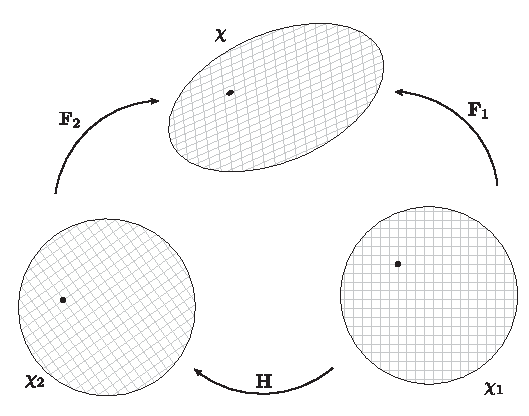
\includegraphics[width=0.7\linewidth]{figure/assunzioni_costitutive/materialSymmetry}
	\caption{A sketch of the regions occupied by a body in a (current) configuration $\chi$ and two reference
		configurations $\chi_1$ and $\chi_2$. The deformation gradient tensors from $\chi_1\to\chi$ and $\chi_2\to\chi$ are $\Fb_1$ and $\Fb_2$.
		The stress at a point  in the deformed configuration is $\Tb$ and is independent of the choice of reference
		configuration.}
	\label{fig:materialsymmetry}
\end{figure}
 
Let \( \widehat{\mathbf{T}}_1 \) and \( \widehat{\mathbf{T}}_2 \) be the stress response functions associated with these two reference configurations.  
Since the Cauchy stress in the current configuration is given both by  
\[
\mathbf{T} = \widehat{\mathbf{T}}_1(\mathbf{F}_1) \quad \text{and} \quad \mathbf{T} = \widehat{\mathbf{T}}_2(\mathbf{F}_2),
\]  
we must have  
\[
\widehat{\mathbf{T}}_2(\mathbf{F}_2) = \widehat{\mathbf{T}}_1(\mathbf{F}_1).
\]

Let \( \mathbf{H} \) be the gradient of the mapping (at \( \xb \)) from the first reference configuration to the second.  
Then \( \mathbf{F}_1 = \mathbf{F}_2 \mathbf{H} \), and so we must have  
\[
\widehat{\mathbf{T}}_2(\mathbf{F}) = \widehat{\mathbf{T}}_1(\mathbf{F} \mathbf{H}) \quad \text{for all nonsingular } \mathbf{F}.
\]  
Thus, if we know the stress response function \( \widehat{\mathbf{T}}_1 \) associated with one reference configuration,  
and the mapping \( \mathbf{H} \) from it to another reference configuration,  
the stress response function in the second reference configuration can be determined from the preceding equation.  

If the two reference configurations happen to be such that  
\[
\widehat{\mathbf{T}}_1(\mathbf{F}) = \widehat{\mathbf{T}}_2(\mathbf{F}) \quad \text{for all nonsingular } \mathbf{F},
\]  
then these two reference configurations have the same stress response functions; see Figure~\ref{fig:materialsymmetry1}. 

\begin{figure}
	\centering
	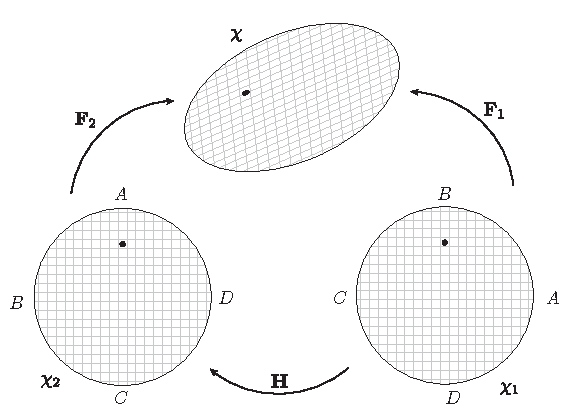
\includegraphics[width=0.7\linewidth]{figure/assunzioni_costitutive/materialSymmetry1}
	\caption{A sketch of the regions occupied by a body in a (deformed) configuration \( \chi \) and two reference configurations \( \chi_1 \) and \( \chi_2 \). The locations of four material points \( A, B, C, D \) in the two reference configurations are shown. Note the symmetry between the reference configurations \( \chi_1 \) and \( \chi_2 \), even though they are distinct. The transformation \( \Hb \) from \( \chi_1 \rightarrow \chi_2 \) preserves the symmetry of the material.}
	\label{fig:materialsymmetry1}
\end{figure}
 
Consider the set of all tensors \( \mathbf{H} \) that take \( \chi_1 \) to a configuration with the identical stress response function.  
This set is  
\[
\left\{ \mathbf{H} : \det \mathbf{H} \neq 0,\ \widehat{\mathbf{T}}(\mathbf{F}) = \widehat{\mathbf{T}}(\mathbf{F} \mathbf{H})\ \text{for all nonsingular } \mathbf{F} \right\}.
\]


This is the set of transformations of the reference configuration that leave the stress response  
function unchanged.  

Next, recall that the mass densities \( \rho_1 \) and \( \rho_2 \) in the two reference configurations are  
related by  
\[
\rho_2 = \rho_1 |\det \mathbf{H}|.
\]  
The mass densities in the two reference configurations are identical if \( |\det \mathbf{H}| = 1 \).  

We say that two configurations are \emph{mechanically indistinguishable} from each other  
if their mass densities and stress response functions coincide.  
Thus, in order to study mechanically indistinguishable configurations,  
we must restrict attention to tensors \( \mathbf{H} \) whose determinant is \( \pm 1 \).  
(If \( \det \mathbf{H} = -1 \), such a tensor could not be the deformation gradient of  
an actual deformation, since \( \det \mathbf{H} > 0 \) is required.  
However, we admit such tensors in our discussion of symmetry,  
as we wish to include reflection tensors among the set of permissible symmetry transformations.)  

A tensor with determinant equal to \( \pm 1 \) is said to be \emph{unimodular}.
The set of all tensors with \(\det\mathbf{H} = \pm 1\) forms the \emph{unimodular group}
\[
\Uc \;=\; \bigl\{\mathbf{H} : \det\mathbf{H} = \pm 1\bigr\}.
\]

In view of the two preceding observations we consider the set of tensors  
\begin{definition}

\begin{equation}\label{symgr}
	\Gc \;=\; \bigl\{\mathbf{H} \in \Uc,\;
\widehat{\mathbf{T}}(\mathbf{F}) = \widehat{\mathbf{T}}(\mathbf{F}\mathbf{H})
\;\text{for all nonsingular } \mathbf{F}\bigr\}.
\end{equation}

\end{definition}

The set \(\Gc\) characterizes all configurations that are mechanically indistinguishable from
\(\chi_1\); it is called the \emph{material symmetry group} of the configuration \(\chi_1\).

Symmetry is a property of a configuration: in general, the same body may possess
different symmetries in different configurations.  
Symmetry transformations are precisely those that leave the “material micro\-structure”
invariant.

From~\eqref{symgr} one can show that  
\begin{enumerate}
	\item  if \(\mathbf{H}_1 \in \Gc\) and \(\mathbf{H}_2 \in \Gc\) then \(\mathbf{H}_1\mathbf{H}_2 \in \Gc\); and  
\item  if \(\mathbf{H} \in \Gc\) then \(\mathbf{H}^{-1} \in \Gc\). 
\end{enumerate} 
Therefore \(\Gc\) is a group.\footnote{That is, \(\Gc\) is closed under multiplication and inversion.}

\medskip
We could equally well base the symmetry discussion on the free-energy potential
\(\widehat{\psi}(\mathbf{F})\), in which case  
\[
\Gc \;=\; \bigl\{\mathbf{H} : \det\mathbf{H} = \pm 1,\;
\widehat{\psi}(\mathbf{F}) = \widehat{\psi}(\mathbf{F}\mathbf{H})
\;\text{for all nonsingular } \mathbf{F}\bigr\}
\]
would describe the symmetry of a configuration.  
%(The reader may verify the relation between the two definitions, recalling that
\(\widehat{\mathbf{T}}(\mathbf{F}) = \rho_0 J^{-1}\,\widehat{\psi}_{\mathbf{F}}(\mathbf{F})\,\mathbf{F}^\top\).)

\medskip

From \eqref{symgr}  it follows that the material symmetry group is a subset of the unimodular group,
\[
\Gc \;\subset\; \Uc. 
\]

In principle, \(\Gc\) may coincide with any subgroup of \(\Uc\).
Two notable subgroups are the set of orthogonal tensors Orth and the set of all rotations about a fixed axis.
Frequently, \(\Gc\) consists of selected rotations and/or reflections.

Using material symmetry together with frame indifference,
one can show that 
\begin{definition}

\begin{equation}\label{matsym}
\Qb\in\Gc \qquad \Longleftrightarrow\qquad	\widehat{\mathbf{T}}\bigl(\mathbf{Q}\mathbf{F}\mathbf{Q}^\top\bigr)
\;=\;
\mathbf{Q}\,\widehat{\mathbf{T}}(\mathbf{F})\,\mathbf{Q}^\top
\quad\text{for all nonsingular } \mathbf{F}, 
\end{equation}

\end{definition}
or, equivalently, in terms of the free energy,
\[
\widehat{\psi}\bigl(\mathbf{Q}\mathbf{F}\mathbf{Q}^\top\bigr)
\;=\;
\widehat{\psi}(\mathbf{F})
\quad\text{for all nonsingular } \mathbf{F}.
\]

In order to prove \eqref{matsym}, we  will proceed in steps.
\begin{enumerate}
	\item ($\Rightarrow$) Assume $\mathbf{Q} \in \mathcal{G}$ and that the frame indifference holds:
	\begin{equation}\label{FI1}
		\widehat{\Tb}(\Qb\Fb)=\Qb\widehat{\Tb}(\Fb)\Qb^\top.
	\end{equation}
Let us define $\Gb=\Fb\Qb^\top$, so that $\Qb\Gb=\Qb\Fb\Qb^\top$. From the frame indifference \eqref{FI1}, we get
\begin{equation}\label{FI2}
	\widehat{\Tb}(\Qb\Gb)=\Qb\widehat{\Tb}(\Gb)\Qb^\top;
\end{equation}
since $\Qb\in\Gc$ by hypothesis,
\begin{equation}
	\widehat{\Tb}(\Gb)=	\widehat{\Tb}(\Gb\Qb)=\widehat{\Tb}(\Fb).
\end{equation}
Therefore \eqref{FI2}  and the definition of $\Gb$ imply
\begin{equation}\label{mats}
		\widehat{\Tb}(\Qb\Fb\Qb^\top)=\Qb\widehat{\Tb}(\Fb)\Qb^\top.
\end{equation}
We have then proved  that $\Qb\in\Gc$ implies \eqref{mats}.
\item ($\Leftarrow$) Assume $	\widehat{\Tb}(\Qb\Fb\Qb^\top)=\Qb\widehat{\Tb}(\Fb)\Qb^\top$ and that the the frame indifference \eqref{FI1} holds . Let now $\Gb=\Fb\Qb$, so that $\Fb=\Gb\Qb^\top$. Because of the hypothesis,
\begin{equation}
	\widehat{\Tb}(\Qb\Gb\Qb^\top)=\Qb\widehat{\Tb}(\Gb)\Qb^\top \qquad \Longrightarrow\qquad 	\widehat{\Tb}(\Qb\Fb)=\Qb\widehat{\Tb}(\Fb\Qb)\Qb^\top.
\end{equation}
By the frame indifference \eqref{FI1} applied to the lhs,  this is equivalent to 
\begin{equation}
\Qb\widehat{\Tb}(\Fb)\Qb^\top=\Qb\widehat{\Tb}(\Fb\Qb)\Qb^\top, 
\end{equation}
or equivalently,
\begin{equation}
\widehat{\Tb}(\Fb)=\widehat{\Tb}(\Fb\Qb).
\end{equation}
We therefore conclude that $\Qb\in\Gc$.
\end{enumerate}

\begin{remark}
	As noted earlier, symmetry is fundamentally a property of a particular configuration of a body. However, when the context is clear and there is no risk of misunderstanding, we will adopt the common (though imprecise) practice of attributing symmetry to the material itself. For example, we will refer to an ``isotropic material'' to mean that the material is considered in a configuration where it exhibits isotropy, and similarly for other symmetry types.
\end{remark}

\subsection{ Examples of Material Symmetry Groups}
\begin{enumerate}
	\item The largest possible material symmetry group is the unimodular group itself:
	\[
	\mathcal{G} = \mathcal{U}.
	\]
	If the material symmetry group of a certain configuration of a body is the unimodular group, one can show that
	\[
	\widehat{\mathbf{T}}(\mathbf{F}) = f(\det \mathbf{F}) \, \mathbf{I},
	\]
	i.e., the Cauchy stress is hydrostatic and depends on the deformation only through the Jacobian $\det \mathbf{F}$. Thus, the body responds as a fluid. If the material symmetry group in one configuration is $\mathcal{U}$, then it is $\mathcal{U}$ in every configuration. Therefore, if the body behaves as a fluid in one configuration, it behaves as a fluid in all configurations.
\item Let $\mathbf{R}^\varphi_\eb$ denote the rotation through an angle $\varphi$ about an axis $\eb$. The set of all such rotations about a fixed axis $\eb$,
\[
\left\{ \mathbf{R}^\varphi_\eb \mid 0 \leq \varphi \leq 2\pi \right\},
\]
forms a group. If the material symmetry group coincides with this group, we say that the body is \textit{transversely isotropic} about the axis $\eb$ in this reference configuration.
\item If the material symmetry group is generated by $\pi/2$ rotations $\mathbf{R}^{\pi/2}_{\eb_1}$, $\mathbf{R}^{\pi/2}_{\eb_2}$, and $\mathbf{R}^{\pi/2}_{\eb_3}$ about the three orthonormal vectors $\{ \mathbf{e}_1, \mathbf{e}_2, \mathbf{e}_r \}$, then the material is said to be \textit{cubic} in this reference configuration.
\item If $\Gc=$Orth, we say that the body is \textit{isotropic} in this reference configuration.
\end{enumerate}


\section{Isotropic materials}
Up to this point, we have focused on how to characterize a material's symmetry. We now turn to understanding how this symmetry can be used to further simplify the constitutive relations.
Let us consider an isotropic material. In this case $\widehat{\psi}(\Qb\Fb\Qb^\top)=\widehat{\psi}(\Fb)$ for all $\Qb\in$Orth. In this event, one can show that $\widehat{\psi}$ has the representation
\begin{equation}
\widehat{\psi}(\Fb)=\psi (I_1(\Cb), I_2(\Cb), I_3(\Cb)),
\end{equation}
where 
\begin{equation}
	I_1(\Cb) = \text{tr}\, \Cb, \quad I_2(\Cb) = \frac{1}{2} \left[(\text{tr}\, \Cb)^2 - \text{tr}(\Cb^2)\right], \quad I_3(\Cb) = \det \Cb = (\det\Fb)^2=J^2, 
\end{equation}
are the principal scalar invariants of the right Cauchy-Green tensor $\Cb = \Fb^\top \Fb = \Ub^2$. (Recall that the eigenvalues and principal scalar invariants of $\Cb$ and $\Bb = \Fb \Fb^\top = \Vb^2$ coincide.) On differentiating with respect to $\Cb$ we find
\begin{equation}\label{derinv}
	\frac{\partial I_1}{\partial \Cb} = \Ib, \quad \frac{\partial I_2}{\partial \Cb} = I_1 \Ib - \Cb, \quad \frac{\partial I_3}{\partial \Cb} = J^2 \Cb^{-1}.
\end{equation}

In order to determine the stress tensor $\Pb$, we may use \eqref{constP} $\Pb = 2\rho_0 \Fb \partial_\Cb\widehat{\psi}$; and since $\Tb = J^{-1} \Pb \Fb^\top$, it follows that
\begin{definition}
	\[
\Tb = 2\rho_0 J^{-1} \Fb \partial_\Cb\widehat{\psi}\Fb^\top,
\]
\end{definition}
which can be used to find $\Tb$. Using these, together with the chain rule and \eqref{derinv}, lead to the following constitutive relations for an elastic material with respect to an isotropic reference configuration:
\begin{equation}
	\left.
	\begin{aligned}
		\rho_0^{-1} \Tb &= 2J \frac{\partial \psi}{\partial I_3} \Ib + \frac{2}{J} \left( \frac{\partial \psi}{\partial I_1} + I_1 \frac{\partial \psi}{\partial I_2} \right) \Bb - \frac{2}{J} \frac{\partial \psi}{\partial I_2} \Bb^2, \\
		\rho_0^{-1} \Pb &= 2 I_3 \frac{\partial \psi}{\partial I_3} \Fb^{-T} + 2 \left( \frac{\partial \psi}{\partial I_1} + I_1 \frac{\partial \psi}{\partial I_2} \right) \Fb - 2 \frac{\partial \psi}{\partial I_2} \Bb \Fb.
	\end{aligned}
	\right\} 
\end{equation}
Note that for an isotropic material, the principal directions of $\Tb$ and $\Bb$ coincide.


\section{Materials with Internal Constraints}
%Abeyaratne
Thus far, we have assumed that the body under consideration can undergo any motion at all by subjecting it to suitable body forces and surface tractions. In certain circumstances, it is possible, and indeed convenient, to idealize the body such that it can only undergo motions of a certain restricted class. 

For example, a \textit{rigid} body can only undergo rigid motions, i.e., motions in which $\Fb(\mathbf{\xb}, t)$ is independent of $\mathbf{x}$ and is proper orthogonal at all $t$; an \textit{incompressible} body can only undergo volume-preserving motions, i.e., motions in which $\det \Fb(\mathbf{\xb}, t) = 1$; a body which is inextensible in a certain (referential) direction $\mathbf{\eb}$ can only undergo motions in which $|\Fb(\mathbf{x}, t)\mathbf{e}| = 1$ at every particle and instant.

A material is said to be subjected to a \textit{simple internal constraint} if it can only undergo motions in which
\begin{equation}\label{constr}
	\widehat\phi(\Fb(\mathbf{x}, t)) = 0 \quad \text{for all } \mathbf{x} \in \widetilde\Omega, \, t \in [t_0, t_1],
\end{equation}
where the function $\widehat\phi$ describes the constraint. The constraints of rigidity, incompressibility, and inextensibility are described by
\[
\widehat\phi(\Fb) = \Fb^\top \Fb - \Ib, \quad \widehat\phi(\Fb) = \det \Fb - 1, \quad \text{and} \quad \widehat\phi(\Fb) = \Fb\mathbf{\eb} \cdot \Fb\mathbf{\eb} - 1,
\]
respectively.

It is natural to require the constraint \eqref{constr} to be material frame indifferent, i.e., if a deformation gradient tensor $\Fb$ obeys the constraint  \eqref{constr}, a subsequent rigid rotation should not lead to a violation of the constraint. That is, if $\Fb$ obeys  \eqref{constr}, then $\Qb\Fb$ must also satisfy  \eqref{constr} for every rotation $\Qb$. Accordingly, we require that
\[
\widehat\phi(\Fb) = \widehat\phi(\Qb\Fb) \quad \text{for all nonsingular tensors } \Fb \text{ and all rotations } \Qb.
\]
The discussion on objectivity can be readily adapted to the present context to show that  \eqref{constr} is objective if and only if the constraint can be expressed in the form
\begin{equation}
	\phi(\Cb(\mathbf{\xb}, t)) = 0 \quad \text{for all } \mathbf{x} \in \widetilde{\Omega}, \, t \in [t_0, t_1], \tag{8.48}
\end{equation}
where $\Cb = \Fb^\top \Fb$. Observe that the three examples given earlier can be expressed in this form: rigidity as $\Cb = \Ib$, incompressibility as $\det \Cb = 1$, and inextensibility as $\Cb\mathbf{e} \cdot \mathbf{e} = 1$.

We now consider the stresses in a constrained body. In order to explain the basic idea, consider as an example, a sphere composed of an incompressible isotropic material that is subjected to a uniform applied pressure $\pi$ on its boundary. Since the geometry, the material, and the loading are all symmetric, let us restrict attention to spherically symmetric deformations. Thus, the sphere can only become a smaller/larger sphere when $\pi$ is applied. However, due to incompressibility, the sphere cannot remain spherical and change its size.

Thus, irrespective of the value of $\pi$, incompressibility implies that any symmetric deformation of the sphere must be the trivial one: $\widehat{\yb}(\mathbf{x}, t) = \mathbf{x}$ and therefore necessarily $\Fb(\mathbf{x}, t) = \Ib$ no matter what the value of $\pi$. The stress, on the other hand, would certainly depend on the value of the applied pressure $\pi$. Thus, the stress $\Tb$ is not completely determined by the deformation gradient $\Fb$, or equivalently,\textit{ different stress fields can correspond to the same deformation}. 

This contradicts our earlier notion of determinism, according to which the stress is completely determined by the history of the motion until time $t$. We must therefore modify this notion when considering a constrained body.

It is customary to suppose that the stress $\Tb^{(\rm A)}$ can be additively decomposed into two parts: one that is determined by the history of the deformation gradient tensor $\Fb$, and the other, say $\Tb^{(\rm R)}$, that is not. The stress $\Tb^{(\rm R)}$ is assumed to spend no power in any motion consistent with the constraint. Thus, for example, one might have
	\begin{equation}\label{Tar}
	\Tb = \widetilde{\Tb}^{(\rm A)}(\Fb, \dot{\Fb}) + \Tb^{(\rm R)},
\end{equation}
where
\begin{equation}\label{recpow}
	 \Tb^{(\rm R)} \cdot \Db = 0 
\end{equation}
for all stretching tensors $\Db$ consistent with the constraint \eqref{constr}. The stress field $\Tb^{(\rm R)}$ arises in ``\textit{reaction}'' to the constraint and is often referred to as the \textit{reaction stress}. One sometimes refers to $ \widetilde{\Tb}^{(\rm A)}$ and $ \Tb^{(\rm R)}$ as the \textit{active} and \textit{reactive} parts of the stress.

Note that \eqref{recpow} does not hold for all symmetric $\Db$ but only for those that are consistent with the constraint  \eqref{constr}. Thus, we now determine the restriction that the constraint places on the stretching tensor. Differentiating \eqref{constr} with respect to $t$ shows that
\begin{equation}
	\partial_\Cb\phi(\Cb) \cdot \dot{\Cb} = 0. 
\end{equation}
On making use of the kinematic identity $\dot{\Cb} = 2 \Fb^\top \Db \Fb$, we get the following restriction on the possible values of $\Db$:
\begin{equation}\label{ort}
	\Fb \, 	\partial_\Cb\phi(\Cb) \, \Fb^\top \cdot \Db = 0.
\end{equation}
This equation states that $\Db$ is orthogonal to $\Fb \partial_\Cb\phi(\Cb) \Fb^\top$. Equations \eqref{recpow} and \eqref{ort} together state that the tensor $ \Tb^{(\rm R)} $ is orthogonal to every tensor $\Db$ that is orthogonal to $\Fb \partial_\Cb\phi(\Cb)\Fb^\top$. Thus, $\Tb^{(\rm R)} $ must be parallel to $\Fb\partial_\Cb (\Cb) \Fb^\top$, and so there exists a scalar field $\lambda(\mathbf{x}, t)$ such that
\begin{definition}
\begin{equation}\label{reac}
	\Tb^{(\rm R)}  = \lambda \, \Fb \, \partial_\Cb\phi(\Cb) \, \Fb^\top.
\end{equation}
\end{definition}

\vspace{.3cm}

As an example, consider an incompressible body, in which case $\phi(\Cb) = \det \Cb - 1$. Thus,
\[
\partial_\Cb\phi(\Cb) = (\det \Cb) \Cb^{-\top} = \Cb^{-1},
\]
so that \eqref{reac} yields the well-known result
\begin{equation}
	\Tb^{(\rm R)}	 = \lambda \Ib 
\end{equation}
which says that the reaction stress is a pressure.

Similarly, for a body that is inextensible in the referential direction $\mathbf{e}$, one finds that
\begin{equation}
		\Tb^{(\rm R)}= \lambda \, \Fb\mathbf{e} \otimes \Fb\mathbf{e};
\end{equation}
here $	\Tb^{(\rm R)}$ is a uniaxial stress in the fiber direction $\mathbf{e}$.



%
%\newpage
%A material is elastic if
%\begin{enumerate}
%	\item The energy $\psi$ and the stress $\Tb$ depend only on the current value of the deformation and not on its past history or the rate at which the deformation changes. As a consequence, the constitutive equations for energy and stress are of the form
%	\begin{equation}\label{constel}
%	%	\psi = \widehat{\psi}(\Fb), \qquad \Tb = \widehat{\Tb}(\Fb).
%		\psi_{\rm ref}=\widehat{\psi}_{\rm ref}(\Fb), \qquad \Pb=\widehat{\Pb}(\Fb).
%	\end{equation}
%	\item It does not dissipate energy:
%	\begin{equation}
%		\rho\gamma = \Tb \cdot \Db - \rho\dot{\psi} = 0.
%	\end{equation}
%\end{enumerate}
%
%\section{Consequences of frame-indifference}
%%For an elastic body we can give  the free energy and stress when $\Fb$ is known:
%%\begin{equation}\label{consteq}
%%	\begin{aligned}
%%		\psi_{\rm ref}=\widehat{\psi}_{\rm ref}(\Fb), \qquad \Pb=\widehat{\Pb}(\Fb).
%%	\end{aligned}
%%\end{equation}
%Because we have in mind to focus on solids, it is more convenient to work in the referential setting; this is emphasized by the subscript `ref' in those fields that may have referential and current counterparts. 
%
%The response functions $\widehat{\psi}_{\rm ref}$ and $\widehat{\Pb}$ can be use to determine the constitute equations for the Cauchy and second Piola stress:
%\begin{equation}\label{C2Pce}
%	\Tb=\widehat{\Tb}(\Fb)=(\det\Fb)^{-1}\widehat{\Pb}(\Fb)\Fb^\top, \qquad \Sb=\widehat{\Sb}(\Fb)=\Fb^{-1}\widehat{\Pb}(\Fb).
%\end{equation}
%
%We now explore the consequences of the hypotheses  stipulating that
%the constitutive equations be frame-indifferent and compatible with thermodynamics.
%
%Since the deformation gradient transforms according to $\Fb^+=\Qb\Fb$,
%\begin{eqnarray}
%	\widehat{\psi}_{\rm ref}(\Fb)=\widehat{\psi}_{\rm ref}(\Qb\Fb).
%\end{eqnarray}
%From \eqref{Pio} it is easy to see that $\Pb^+=\Qb\Pb$, so that
%\begin{equation}
%	\Pb^+=\widehat{\Pb}(\Fb^+)=\widehat{\Pb}(\Qb\Fb).
%\end{equation}
%
%The response maps $\widehat{\psi}_{\rm ref}$ and $\widehat{\Pb}$ must therefore satisfy
%\begin{equation}
%	\widehat{\psi}_{\rm ref}(\Fb)=\widehat{\psi}_{\rm ref}(\Qb\Fb), \quad \widehat{\Pb}(\Fb)=\Qb^\top\widehat{\Pb}(\Qb\Fb),
%\end{equation}
%for all rotations $\Qb$ and $\Fb$. Fix $\Fb$ and consider the polar decomposition $\Fb=\Rb\Ub$. Since $\Qb$ is arbitrary, we choose $\Qb=\Rb^\top$; hence $\Qb\Fb=\Ub$ and
%\begin{equation}
%	\widehat{\psi}_{\rm ref}(\Fb)=\widehat\psi_{\rm ref}(\Ub), \quad \widehat{\Pb}(\Fb)=\Rb\widehat{\Pb}(\Ub).
%\end{equation}
%Replacing $\Ub$ by $\sqrt{\Cb}$, we may introduce a response function $\widetilde{\psi}_{\rm ref}$ determining the free energy $\psi_{\rm ref}$ as a function of $\Cb$ via
%\begin{equation}
%	\widetilde{\psi}_{\rm ref}(\Cb)=\widehat\psi_{\rm ref}(\sqrt{\Cb}).
%\end{equation}
%Similarly, in view of \eqref{C2Pce}$_2$ for the second Piola stress we find that
%\begin{equation}
%	\Rb\widehat{\Pb}(\Ub)=\Fb\Ub^{-1}\widehat{\Pb}(\Ub)=\Fb\widehat{\Sb}(\Fb)=\Rb\Ub\widehat{\Sb}(\Fb).
%\end{equation} 
%Hence  $\widehat{\Pb}(\Ub)=\Ub\widehat{\Sb}(\Fb)$,
%\begin{equation}
%	\widehat{\Sb}(\Fb)=\Ub^{-1}\widehat{\Pb}(\Ub),
%\end{equation}
%and, replacing $\Ub$ by $\sqrt{\Cb}$, we may introduce a response function $\widetilde{\Sb}$ determining the second Piola stress as a function of $\Cb$:
%\begin{equation}
%	\Sb=\Cb^{-1/2}\widehat{\Pb}(\sqrt{\Cb})=\widetilde{\Sb}(\Cb).
%\end{equation}
%
%If the constitutive equations \eqref{constel} are to be frame-indifferent, the foregoing results show that they must reduce to constitutive equations of the specific form
%\begin{equation}
%	\psi_{\rm ref}=\widetilde{\psi}_{\rm ref}(\Cb), \qquad \Pb=\Fb\widetilde{\Sb}(\Cb).
%\end{equation}
%
%Since the second Piola stress is symmetric, an important consequence of this latter relation is that
%\begin{equation}
%	\Pb\Fb^\top-\Fb\Pb^\top=\Fb\Sb\Fb^\top-\Fb\Sb^\top\Fb^\top=\Fb(\Sb-\Sb^\top)\Fb^\top=\mathbf{0}.
%\end{equation}
%Hence the requirement that the constitutive equations be frame-indifferent implies satisfaction of the moment balance. Granted frame-indifferent constitutive equations, we may therefore neglect the moment balance from further consideration.


\section{Infinitesimal theory}
It is possible to write the constitutive equation for the stress in terms of the displacement $\ub(\xb)=\fb(\xb)-\xb$:
\begin{equation}
\Tb(\yb)=\widehat{\Tb}(\Ib +\Hb(\xb)).
\end{equation}
If $\widehat{\Tb}$ is sufficiently smooth, we may write
\begin{equation}
\Tb(\yb)=\widehat{\Tb}(\Ib)+\partial_\Fb \widehat{\Tb}(\Ib)\,\Hb+o(|\Hb|).
\end{equation}
The term $=\widehat{\Tb}(\Ib)$ represents the stress in the referential configuration, that we assume null. With this, and \eqref{C2Pce}$_1$, we have
\begin{equation}
\Pb(\xb)=\det \Fb(\xb)\, \Tb(\yb) \Fb^{-\top}(\xb)=\det \Fb(\xb)\, \big( \partial_\Fb \widehat{\Tb}(\Ib)\,\Hb+o(|\Hb|) \big) \Fb^{-\top}(\xb).
\end{equation}
If we argument as in chapter \ref{inf}, we deduce that
\begin{equation}
\Pb=(1+\operatorname{tr}\Hb)\,  \big( \partial_\Fb \widehat{\Tb}(\Ib)\,\Hb+o(|\Hb|) \big) (\Ib-\Hb^{-\top})=\partial_\Fb \widehat{\Tb}(\Ib)\,\Hb+o(|\Hb|),
\end{equation}
and then
\begin{definition}
\begin{equation}
\Pb(\xb)=\Tb(\yb)+o(|\Hb|).
\end{equation}
\end{definition}
Therefore, up to infinitesimals of order \( o(|\Hb|) \), the Cauchy stress tensor evaluated at \( \fb(\xb) \) is equal to the Piola stress tensor evaluated at \( \xb \):
Identifying the configuration determined by the deformation \( \fb \) with the reference configuration introduces an error of order \( o(|\Hb|) \). More precisely, up to infinitesimals of order \( o(|\Hb|) \), it is possible to define a stress tensor---still referred to as the Cauchy stress tensor and denoted by \( \Tb \)---on the reference configuration such that:
\begin{enumerate}
	\item  \( \Tb(\xb) = \Tb(\xb) \) for every \( \xb \in \Omega = \kappa(\Bb) \);
	\item  the equilibrium equation  becomes  
	\[
	\operatorname{Div}\Tb(\xb) + \bb(\xb) =\mathbf{0}
	\]  
	for every \( \xb \in \Omega \), where \( \bb \) denotes the body forces per unit volume in the reference configuration;
\item  \( \Tb(\xb)\nb(\xb) \) represents the stress at the point \( \fb(\xb) \) along a surface whose preimage has normal \( \nb \).
\end{enumerate}

For sake of simplicity, \textit{in the following we will just consider the infinitesimal theory}. Therefore, 
 we can write the following constitutive equations:
\begin{equation}
\Tb=\widehat{\Tb}(\Eb), \qquad \psi=\widehat{\psi}(\Eb).
\end{equation}
 Moreover, we set
\begin{equation}
\rho\varepsilon=\bar{\varepsilon}, \quad \rho\eta=\bar{\eta}, \quad \rho\delta=\bar\delta, \quad \rho \psi=\bar{\psi}.
\end{equation}
We will work with the barred quantities, but omit the bars in the notation. Eventually, no difference will be between $\nabla\varphi$, $\grad\varphi$, $\Div\varphi$ and $\dive\varphi$.


\section{Consequences of thermodynamic restrictions}
To understand the consequences of the thermodynamic restrictions, we use the Coleman-Noll procedure. 

Since the process is given by $\psi = \widehat{\psi}(\Eb)$ and $\Tb = \widehat{\Tb}(\Eb)$, equation \eqref{gammael} can be rewritten as
\begin{equation}
	\widehat{\Tb}(\Eb) \cdot \dot{\Eb} - \left(\widehat{\psi}(\Eb)\right)^{\mathop{\vcenter{\hbox{\Large$\cdot$}}}} = 0,
\end{equation}
or, using the chain rule
\begin{equation}\label{Tepsi}
	\left( 	\widehat{\Tb}(\Eb) - \partial_\Eb \widehat{\psi} \right) \cdot \dot{\Eb} = 0.
\end{equation}

This condition must be satisfied for every local continuation of any conceivable process; in particular, we assume that the geometry of the state space is such that a local continuation of any trajectory in the space is accessible.

In other words, for every pair $(\Sc, \dot{\Sc})$, we assume that there exists a trajectory $t \mapsto \Sc(t)$ and an instant of time $t_0$ such that $\Sc(t_0) = \Sc$ and $\dot{\Sc}(t_0) = \dot{\Sc}$.

In this context, this means that equation \eqref{Tepsi} must hold \textit{for every} $\dot{\Eb}$ and therefore
\begin{definition}
	\begin{equation}\label{Tdevpsi}
		\widehat{\Tb}(\Eb) = \partial_\Eb \widehat{\psi}(\Eb).
	\end{equation}
\end{definition}
Such a material is called \textit{hyperelastic}.

For \textit{linear elastic materials}, we consider an expansion of the constitutive response function of stress around a \textit{relaxed} reference configuration, that is, with $\Eb = \mathbf{0}$, $\psi = 0$, and $\Tb = \mathbf{0}$; the requirement that $\Tb$ is zero in the reference configuration is not fundamental and can be removed, leading to materials with self-stresses or residual stresses. Thus, we have
\begin{equation}
	\widehat{\Tb} = \widehat{\Tb}(\mathbf{0}) + \left(\left.\partial_\Eb \widehat{\Tb}(\Eb)\right|_{\Eb = \mathbf{0}}\right)\,\Eb + o(|\mathbf{E}|).
\end{equation}
Since the reference configuration is relaxed, $\widehat{\Tb}(\mathbf{0}) = \mathbf{0}$. Due to equation \eqref{Tdevpsi}, we can write
\begin{equation}
	\left.\partial_\Eb \widehat{\Tb}(\Eb)\right|_{\Eb = \mathbf{0}} = \left.\partial^2_{\Eb \Eb} \widehat{\psi}(\Eb)\right|_{\Eb = \mathbf{0}} =: \Co,
\end{equation}
where we have introduced the elasticity tensor (of fourth order) $\Co$. Neglecting infinitesimals of order $o(|\Eb|)$, we can then write the constitutive response map for stress:
\begin{definition}
	\begin{equation}
		\Tb = \widehat{\Tb}(\Eb) = \Co \Eb, \qquad \qquad (T_{ij} = \Co_{ijhk} E_{kh})
	\end{equation}
\end{definition}
The associated energy, due to equation \eqref{Tdevpsi}, is given by the following constitutive response map:
\begin{definition}
	\begin{equation}
		\psi = \widehat{\psi}(\Eb) = \frac{1}{2} \Co \Eb \cdot \Eb, \qquad \qquad \left(\psi = \frac{1}{2} \Co_{ijhk} E_{ij} E_{hk} \right)
	\end{equation}
\end{definition}

Since
\begin{equation}
	\frac{\partial^2 \widehat{\psi}(\Eb)}{\partial E_{ij} \partial E_{hk}} = \frac{\partial^2 \widehat{\psi}(\Eb)}{\partial E_{hk} \partial E_{ij}},
\end{equation}
it follows that the components $\Co_{ijhk}$ of $\Co$ possess the so-called \textit{major symmetries}:
\begin{definition}
	\begin{equation}
		\Co_{ijhk} = \Co_{hkij}.
	\end{equation}
\end{definition}

Furthermore, since $\Tb \in \Sym$,
\begin{equation}
	T_{ij} = \Co_{ijhk} E_{hk} = T_{ji} = \Co_{jihk} E_{hk},
\end{equation}
the components $\Co_{ijhk}$ of $\Co$ also possess the so-called \textit{minor symmetries}:

\begin{definition}
	\begin{equation}
		\Co_{ijhk} = \Co_{jihk}.
	\end{equation}
\end{definition}

For the minor symmetries, the components of $\Co$ are at most $6^2 = 36$; indeed, considering $\Co_{ijhk}$, the pair $ij$, due to symmetry, produces at most 6 independent components, and the same holds for the pair $hk$.

The major symmetry further reduces the number of components to at most $36 - 15 = 21$.


\section{Material symmetries}
We say that $\Qb$ represents a material symmetry if rotations or reflections of the material by $\Qb$ cannot be detected through stress-strain experiments.

Suppose we have a material made of a matrix in which fibers are embedded in the direction $\eb_1$. Imagine measuring the stress required to produce an extension $\varepsilon$ in the $\eb_1$ direction, that is, by imposing the strain
\begin{equation}
	\Eb =\varepsilon\,\eb_1\otimes\eb_1.
\end{equation}
Now imagine measuring the stress required to produce an extension equal to $\varepsilon$ but in a direction rotated by $\Qb=\Rb (\pi/2, \eb_3)$, that is, by $\pi/2$ about $\eb_3$:
\begin{equation}
	\Eb ^\Qb =\varepsilon\, \eb_2 \otimes \eb_2= \varepsilon\,\Qb \eb_1 \otimes \Qb \eb_1.
\end{equation}

Clearly, we expect the stress measured in the second experiment to be different from the first one, and thus $\Qb$ does \textit{not} represent a material symmetry. A rotation by $\pi$, on the other hand, would not be detectable, since the material would be indistinguishable from the original one when rotated by $\pi$; in this case, $\Rb(\pi, \eb_3)$ would represent a material symmetry.

Let us now clarify what we mean by measuring the same stress in two different experiments, like those just described.

In a uniaxial test, a strain $\Eb=\varepsilon\,\eb_1\otimes\eb_1$ corresponds to a stress
\begin{equation}
	\Tb =\sigma \eb_1\otimes\eb_1.
\end{equation}
Now suppose we carry out the same experiment in a direction rotated by $\Qb=\Rb (\pi/2, \eb_3)$, applying an extension $\varepsilon$ in the $\eb_2$ direction, i.e., $\Eb^\Qb=\varepsilon\eb_2\otimes\eb_2$, and we measure the resulting stress:
\begin{equation}
	\Tb^\Qb =\sigma^\Qb\eb_2\otimes \eb_2.
\end{equation}
Clearly, the stress is the same if
\begin{equation}
	\sigma=\sigma^\Qb
\end{equation}
and not when $\Tb =\Tb ^\Qb$.

Let us generalize this through the example of uniaxial tension. By the spectral theorem, we can represent $\Eb$ as
\begin{equation}\label{espettr1}
	\Eb=\sum_{i=1}^{3}\varepsilon_i\, \vb_i\otimes \vb_i,
\end{equation}
where $(\varepsilon_i, \vb_i)$ are the eigenpairs of $\Eb$. The rotated strain $\Eb^\Qb$ is a strain with the same extensions $\varepsilon_i$ but in the directions rotated by $\Qb$:
\begin{equation}
	\Eb^\Qb\coloneqq \sum_{i=1}^{3}\varepsilon_i\, \Qb\vb_i\otimes \Qb\vb_i,
\end{equation}
that is,\footnote{Here we use the property valid for all $\Ab, \Bb\in$ Lin, $\ab, \bb \in \Vc$:
	\begin{equation}
		\Ab(\ab\otimes\bb)\Bb=\Ab \ab \otimes \Bb^\top \bb.
\end{equation}}
\begin{equation}
	\Eb^\Qb=\Qb\sum_{i=1}^{3}\varepsilon_i\, \vb_i\otimes \vb_i \Qb ^\top = \Qb \Eb \Qb^\top.
\end{equation}
Let us denote by 
\begin{equation}
	\Tb \coloneqq\Co \Eb, \qquad \Tb^\Qb\coloneqq \Co \Eb^\Qb=\Co (\Qb \Eb \Qb^\top)
\end{equation}
the responses to the strains $\Eb$ and $\Eb^\Qb$. Since $\Tb$ and $\Tb^\Qb$ are symmetric, we can write their spectral representation:
\begin{equation}
	\Tb=\sum_{i=1}^{3}\sigma_i\, \tb_i\otimes \tb_i, \qquad 	\Tb^\Qb=\sum_{i=1}^{3}\sigma_i\, \tb^\Qb_i\otimes \tb^\Qb_i.
\end{equation}
We will say that $\Qb\in$ Orth is a material symmetry if
\begin{equation}
	\sigma_i=\sigma_i^\Qb, \qquad \tb_i^\Qb=\Qb \tb_i,
\end{equation}
that is, if $\Eb$ and $\Eb^\Qb$ produce the same principal stresses in directions rotated by $\Qb$. 

Therefore, if $\Qb$ is a symmetry
\begin{equation}
	\Co(\Qb\Eb \Qb^\top)=\Co \Eb^\Qb=\Tb^\Qb=\sum_{i=1}^{3}\sigma_i\, \tb^\Qb\otimes \tb^\Qb=\Qb \left(  \sum_{i=1}^{3}\sigma_i\, \tb_i\otimes \tb_i \right)\Qb^\top=\Qb \Tb \Qb^\top=\Qb\Co \Eb \Qb^\top.
\end{equation}
We conclude that $\Qb\in$ Orth is a material symmetry if
\begin{definition}
	\begin{equation}
		\Co(\Qb\Eb \Qb^\top)=\Qb \Co \Eb \Qb ^\top \qquad \forall \Eb \in \Sym,
	\end{equation}
\end{definition}
that is,
\begin{definition}
	\begin{equation}
		\widehat{\Tb}(\Qb \Eb \Qb ^\top)=\Qb \widehat{\Tb}(\Eb)\Qb ^\top, \qquad \forall \Eb \in \Sym.
	\end{equation}
\end{definition}

The set
\begin{equation}
	\Gc =\{ \Qb \in {\rm Orth}\, :\, \widehat{\Tb}(\Qb \Eb \Qb ^\top)=\Qb \widehat{\Tb}(\Eb)\Qb ^\top, \quad \forall \Eb \in \Sym  \}
\end{equation}
is called the \textit{material symmetry group}, and its elements are the material symmetries.

\begin{exercise}
	Let $\mathcal{G}_{\mathbb{C}}$ be the symmetry group of an elastic material and $\psi=\widehat\psi(\Eb)$ the elastic energy density
	\begin{equation}
		\psi=\widehat\psi(\Eb)=\frac12 \Co\Eb\cdot\Eb.
	\end{equation}
	
	Show that, for every $\Qb\in\mathcal{G}_{\mathbb{C}}$,
	\begin{equation}
		\widehat\psi(\Eb)=	\widehat\psi(\Qb\Eb\Qb^\top).
	\end{equation}
	
	\begin{svolgimento}
		We have
		\begin{equation}
			\widehat{\psi}(\Eb)=\frac{1}{2}\widehat{\Tb}(\Eb)\cdot \Eb, \qquad \widehat{\psi}(\Qb\Eb\Qb^\top)=\frac{1}{2}\widehat{\Tb}(\Qb\Eb\Qb^\top)\cdot \Qb\Eb\Qb^\top.
		\end{equation}
		Since $\Qb \in \mathcal{G}_{\mathbb{C}}$
		\begin{equation}
			\widehat{\Tb}(\Qb\Eb\Qb^\top)=\Qb\widehat{\Tb}(\Eb)\Qb^\top,
		\end{equation}
		and thus
		\begin{equation}
			\widehat{\psi}(\Qb\Eb\Qb^\top)=\frac12\Qb\widehat{\Tb}(\Eb)\Qb^\top\cdot  \Qb\Eb\Qb^\top=\frac12 \Qb^\top\Qb \widehat{\Tb}(\Eb)\cdot \Eb \Qb^\top\Qb=\frac{1}{2}\widehat{\Tb}(\Eb)\cdot \Eb=\widehat{\psi}(\Eb).
		\end{equation}
		The result shows the obvious invariance of the energy with respect to material symmetry transformations.
	\end{svolgimento}
	
\end{exercise}


\section{Isotropic materials}
A material is isotropic if its elastic response is the same in all directions, namely
\begin{equation}
	\Gc ={\rm Orth},
\end{equation}
and therefore
\begin{equation}
	\widehat{\Tb}(\Qb \Eb \Qb ^\top)=\Qb \widehat{\Tb}(\Eb)\Qb ^\top, \qquad \forall \Eb \in \Sym, \Qb \in {\rm Orth}.
\end{equation}

A relevant property of an isotropic material, known as \textit{coaxiality}, is that
when it is subjected to deformation, the directions in which maximum and minimum strains occur (principal strain directions) are the same as those in which maximum and minimum stresses develop (principal stress directions). In other words, if one observes an isotropic material undergoing loading, the directions along which strains are maximum (e.g., stretching or compression) coincide with those along which stresses are maximum. This behavior reflects the uniformity of the material in all spatial directions. For example, if a material elongates along a principal direction, the stress causing this deformation will be oriented in the same direction.

We now state more precisely the 
\begin{definition}
 \textit{\textbf{Coaxiality Theorem}}.	Let $\widehat{\Tb}(\Eb)$ be isotropic, that is
	\begin{equation}
		\widehat{\Tb}(\Qb \Eb \Qb ^\top)=\Qb \widehat{\Tb}(\Eb)\Qb ^\top, \qquad \forall \Eb \in \Sym, \Qb \in {\rm Orth},
	\end{equation}
	then every eigenvector of $\Eb\in \Sym$ is also an eigenvector of $\widehat{\Tb}(\Eb)$.
\end{definition}

Let us prove the theorem. Let $\vb$ be an eigenvector of $\Eb$. We choose the basis
\begin{equation}
	\{\eb_1\equiv \vb, \eb_2, \eb_3  \},
\end{equation}
so that $\Eb$ admits the following spectral representation:
\begin{equation}
	\Eb =\varepsilon_1\, \vb \otimes \vb +\varepsilon_2 \eb_2 \otimes \eb_2+ \varepsilon_3 \eb_3 \otimes \eb_3.
\end{equation}
Let $\Rb_\vb\in$ Orth be the reflection with respect to a plane normal to $\vb$; a vector $\ab$ parallel to $\vb$ is mapped to $\Rb_\vb\ab=-\ab$, while a vector $\bb$ orthogonal to $\vb$ is mapped to $\Rb_\vb\bb=\bb$. In particular,
\begin{equation}
	\Rb_\vb\vb =-\vb, \qquad \Rb_\vb\eb_2=\eb_2, \qquad \Rb_\vb\eb_3=\eb_3
\end{equation}
and therefore
\begin{equation}\label{RvE}
	\Rb_\vb\Eb \Rb_\vb^\top=\Eb.
\end{equation}
Since $\widehat{\Tb}$ is isotropic, by choosing $\Qb=\Rb_\vb$, we get
\begin{equation}
	\widehat{\Tb}(\Rb_\vb\Eb \Rb_\vb^\top)=\Rb_\vb\widehat{\Tb}(\Eb)\Rb_\vb^\top,
\end{equation}
but from \eqref{RvE}, we have
\begin{equation}
	\widehat{\Tb}(\Eb)=\Rb_\vb\widehat{\Tb}(\Eb)\Rb_\vb^\top.
\end{equation}
We now determine the image under the reflection $\Rb_\vb$ of the stress vector on a plane normal to $\vb$:
\begin{equation}
	\Rb_\vb\widehat{\Tb}(\Eb)\vb=	\Rb_\vb\widehat{\Tb}(\Eb)\Ib\vb=\Rb_\vb\widehat{\Tb}(\Eb)\Rb_\vb^\top\Rb_\vb \vb=\widehat{\Tb}(\Eb)\Rb_\vb \vb=-\widehat{\Tb}(\Eb)\vb,
\end{equation}
and thus
\begin{equation}
	\Rb_\vb\widehat{\Tb}(\Eb)\vb=-\widehat{\Tb}(\Eb)\vb.
\end{equation}
This is only possible if the stress vector $\widehat{\Tb}(\Eb)\vb$ is parallel to $\vb$:
\begin{equation}
	\widehat{\Tb}(\Eb)\vb=\lambda \vb, \quad \lambda\in \Ro,
\end{equation}
that is, $\vb$ is an eigenvector of $\widehat{\Tb}(\Eb)$, which concludes the proof.

\vspace{.3cm}

For an isotropic material it is possible to state a theorem, which gives an explicit form of $\widehat{\Tb}(\Eb)$:
\begin{definition}
 \textit{\textbf{Representation Theorem}}.	A linear elastic material is isotropic if and only if there exist two constants $\mu$ and $\lambda$ (called Lamé constants) such that
	\begin{equation}
		\widehat{\Tb}(\Eb)=\Co \Eb =2 \mu \Eb +\lambda(\operatorname{tr} \Eb )\Ib,
	\end{equation}
	for every $\Eb\in\Sym$.
\end{definition}

The proof relies on the coaxiality theorem and on a consequence of the spectral theorem. Since $\Eb\in \Sym$, it admits the following spectral representation:
\begin{equation}\label{espettr}
	\Eb=\sum_{i=1}^{3}\varepsilon_i\, \vb_i\otimes \vb_i.
\end{equation}
The property of interest is the following: let $\varepsilon_1$ be the eigenvalue of $\Eb\in \Sym$ associated with $\vb$, with algebraic multiplicity 1, and let $\varepsilon_2$ be the eigenvalue with algebraic multiplicity 2. Then every vector orthogonal to $\vb$ is an eigenvector:
\begin{equation}
	\Eb=\varepsilon_1 \vb \otimes \vb + \varepsilon_2 (\wb_1\otimes\wb_1+\wb_2\otimes\wb_2),
\end{equation} 
with $\wb_1\cdot\vb = \wb_2\cdot \vb=\wb_1\cdot\wb_2=0$.
It follows that
\begin{equation}
	\begin{aligned}
		\Eb &=\varepsilon_1 \vb \otimes \vb+\varepsilon_2(\wb_1\otimes\wb_1\wb_2\otimes\wb_2+\vb_1\otimes\vb_1)-\varepsilon_2\vb \otimes \vb,
	\end{aligned}
\end{equation}
that is 
\begin{definition}
	\begin{equation}\label{Evv}
		\begin{aligned}
			\Eb  =\lambda\, \Ib +2\mu \,\vb \otimes \vb,
		\end{aligned}
	\end{equation}
\end{definition}
with $\lambda\coloneqq \varepsilon_2$ and $\mu\coloneqq(\varepsilon_1-\varepsilon_2)/2$.

\vspace{.3cm}

We now have all the ingredients to prove the Representation Theorem. Observe that for every $\vb$ with $|\vb|=1$, the tensor $\vb \otimes \vb$ has eigenvector $\vb$ (with eigenvalue 1) and every vector $\wb$ orthogonal to $\vb$ (with eigenvalue 0); indeed
\begin{equation}
	(\vb \otimes \vb)\,\vb=\vb, \qquad (\vb \otimes \vb)\,\wb=\mathbf{0}.
\end{equation}
By the coaxiality theorem, $\vb$ is also an eigenvector of $\widehat{\Tb}(\vb \otimes\vb)$. Then, by property \eqref{Evv}, there exist two functions $\lambda(\vb)$ and $\mu (\vb)$ such that
\begin{equation}\label{Tbvv}
	\widehat{\Tb}(\vb \otimes \vb)=\lambda(\vb)\, \Ib+2\mu (\vb) \vb \otimes \vb.
\end{equation}

Let $\wb =\Qb \vb$, with $\Qb \in$ Orth; since $\widehat{\Tb}$ is isotropic,
\begin{equation}
	\Qb \widehat{\Tb}(\vb \otimes \vb)\Qb ^\top=\widehat{\Tb}(\Qb \vb \otimes \Qb \vb)=\widehat{\Tb}(\wb \otimes \wb);
\end{equation}
therefore
\begin{equation}
	\Qb \widehat{\Tb}(\vb \otimes \vb)\Qb ^\top-\widehat{\Tb}(\wb \otimes \wb)=\mathbf{0}.
\end{equation}
In light of \eqref{Tbvv}, we then write
\begin{equation}
	\lambda(\vb) \,\Ib+2\mu(\vb) \Qb \vb \otimes \Qb \vb -\lambda(\wb) \Ib -2\mu (\wb)\, \wb \otimes \wb =\mathbf{0},
\end{equation}
that is,
\begin{equation}
	\Big(  \lambda(\vb)-\lambda(\wb) \Big)\,\Ib+2\Big(  \mu (\vb)-\mu (\wb) \Big)\,\wb \otimes \wb.
\end{equation}
Since $\Ib$ and $\wb \otimes \wb$ are linearly independent, this condition implies that
\begin{equation}
	\lambda(\vb)=\lambda(\wb), \qquad \mu(\vb)=\mu(\wb), \qquad \forall \vb, \wb
\end{equation}
that is, $\lambda$ and $\mu$ are constants. Hence,
\begin{equation}
	\widehat{\Tb}(\vb \otimes \vb)=\lambda\, \Ib+2\mu (\vb \otimes \vb).
\end{equation}
We now use the spectral representation \eqref{espettr}:
\begin{equation}
	\widehat{\Tb}(\Eb)=\sum_{i=1}^3 \varepsilon_i \widehat{\Tb}(\vb_i\otimes \vb_i)=2\mu \sum_{i=1}^3 \varepsilon_i \vb_i \otimes \vb_i +\lambda\sum_{i=1}^3 \varepsilon_i \Ib=2\mu \Eb +\lambda(\operatorname{tr}\Eb )\Ib,
\end{equation}
which concludes the proof.


\section{Interpretation of the Elastic Constants}
In engineering practice, the two Lamé constants are generally replaced by other equivalent constants that have a more significant mechanical interpretation. In particular, we introduce the constants
\begin{equation}
	E=\frac{(2\mu+3\lambda)\mu}{\mu+\lambda}, \qquad \nu = \frac{\lambda}{2(\mu+\lambda)};
\end{equation}
the constant $\mu$ is often denoted by the letter $G$, and so we shall do; it then follows that
\begin{equation}
	G=\frac{E}{2(1+\nu)}.
\end{equation}

With these new constants, the constitutive relation becomes
\begin{definition}
	\begin{equation}\label{const3D}
		\mathbf{T}=\Co \Eb=\frac{E}{1+\nu}{\left(\mathbf{E}+\frac{\nu}{1-2\nu}(\operatorname{tr}\mathbf{E})\mathbf{I}\right)}.
	\end{equation}
\end{definition}

To invert the constitutive relation, it is convenient to determine its trace:
\begin{equation}
	\operatorname{tr}\Tb=\frac{E}{1-2\nu} \operatorname{tr}\Eb \qquad \Longrightarrow \operatorname{tr}\Eb =\frac{1-2\nu}{E}\operatorname{tr}\Tb,
\end{equation} 
which can be inserted into \eqref{const3D} to find:
and the inverse constitutive relation:
\begin{definition}
	\begin{equation}\label{costinv}
		\Eb=\mathbb{C}^{-1}\mathbf{T}=\frac{1+\nu}{E}\mathbf{T}-\frac{\nu}{E}(\operatorname{tr}\mathbf{T})\mathbf{I}.
	\end{equation}
\end{definition}
The role of the elastic moduli becomes clear when one imagines performing certain typical experiments, in each of which one or the other modulus is evidently involved. In the first two experiments we will consider, we record the stress corresponding to a given strain according to the constitutive relation \eqref{const3D}; in the third experiment, the stress is prescribed and the corresponding strain is computed using \eqref{costinv}.

\vspace{.3cm}

\begin{enumerate}
	\item \textit{Pure shear}\\
	We recall  that a pure shear strain has the form
	\begin{equation}
		\Eb=\frac{\gamma}{2}(\mb\otimes \nb+\nb\otimes \mb),
	\end{equation}
	with $\mb$ and $\nb$ orthogonal. The resulting stress, according to \eqref{const3D}, is then
	\begin{equation}
		\Tb=\frac{\gamma}{2}2G(\mb\otimes \nb+\nb\otimes \mb);
	\end{equation}
	thus the coefficient
	\begin{equation}
		2G=\frac{\nb \cdot \Tb \mb}{\nb \cdot \Eb \mb}
	\end{equation}
	measures the shear stress necessary to maintain unit shear strain; for this reason it is called the \textit{shear modulus}.
	
	\item \textit{Uniform dilatation}\\
	In this experiment,
	\begin{equation}
		\Eb=\kappa \Ib,
	\end{equation}
	which leads to a stress
	\begin{equation}
		\Tb=\frac{E}{1-2\nu}\kappa \,\Ib,
	\end{equation}
	that is, a uniform tensile stress of intensity $\pi=\frac{E}{1-2\nu}\kappa $. The ratio between this stress and the volume change given by the trace of $\Eb$ defines the \textit{bulk modulus}
	\begin{equation}\label{compr}
		\beta\coloneqq \frac{\pi}{\operatorname{tr}\Eb}=\frac{E}{3(1-2\nu)}.
	\end{equation}
	
	\item \textit{Uniaxial tension}\\
	In this experiment
	\begin{equation}
		\Tb = \sigma\nb \otimes \nb,
	\end{equation}
	which corresponds to a strain given, in light of \eqref{costinv}, by
	\begin{equation}
		\Eb=\sigma\left(\frac{1+\nu}{E}\nb \otimes \nb-\frac{\nu}{E}\Ib  \right).
	\end{equation}
	The ratio between the stress in the direction $\nb$ and the specific elongation in the same direction is
	\begin{equation}
		\frac{\Tb \nb \cdot \nb}{\Eb \nb \cdot \nb}=E.
	\end{equation}
	The constant $E$ is called the \textit{Young's modulus} and thus measures the stress required to cause unit specific elongation.
	
	The meaning of the constant $\nu$, called the \textit{Poisson's ratio}, becomes evident by measuring the ratio between the transverse and axial strains in a uniaxial tension experiment:
	\begin{equation}
		\nu=-\frac{\Eb \mb \cdot \mb}{\Eb \nb \cdot \nb},
	\end{equation}
	where $\mb$ is orthogonal to $\nb$.
\end{enumerate}

\vspace{.3cm}
The physical dimensions of the elastic constants are
\begin{equation}
	[E]=[G]=\frac{F}{L^2}, \quad [\nu]=-.
\end{equation}
Generally, the Young’s modulus and the shear modulus are expressed in ${\rm N}/{\rm m}^2={\rm Pa}$.

\vspace{.3cm}

The elastic constants cannot take arbitrary values; they must satisfy the conditions
\begin{equation}
	E>0, \quad G>0, \qquad -1<\nu<\frac12.
\end{equation}
The reason is that the elastic energy must be positive. First, observe that, thanks to the constitutive relation \eqref{const3D}, the elastic energy can be expressed in terms of $\Tb$:
\begin{equation}
	\psi=\widehat\psi(\Eb)=\frac12 \Co \Eb \cdot \Eb =\frac 12 \Tb \cdot \Co^{-1}\Tb=:\widetilde{\psi}(\Tb).
\end{equation}

We decompose $\Tb$ as follows:
\begin{equation}
	\Tb=\operatorname{sph}\Tb+\operatorname{dev}\Tb, 
\end{equation}
where the \textit{spherical} part $\operatorname{sph}\Tb$ and the \textit{deviatoric} part $\operatorname{dev}\Tb$ are defined as
\begin{equation}
	\operatorname{sph}\Tb\coloneqq \frac{1}{3}(\operatorname{tr}\Tb)\, \Ib, \qquad \operatorname{dev}\Tb\coloneqq \Tb-	\operatorname{sph}\Tb.
\end{equation}

Doing so, using \eqref{costinv},
\begin{equation}
	\Eb=\Co ^{-1}\Tb =\frac{1+\nu}{E}(\operatorname{sph}\Tb+\operatorname{dev}\Tb)-\frac{\nu}{E}(3	\operatorname{sph}\Tb)\mathbf{I}=\frac{1-2\nu}{E}	\operatorname{sph}\Tb+\frac{1+\nu}{E}	\operatorname{dev}\Tb.
\end{equation}
The elastic energy is then positive if
\begin{equation}\label{ensf}
	\widetilde{\psi}(\Tb)=\frac{1}{2}\left( \frac{1-2\nu}{E}	|\operatorname{sph}\Tb|^2+\frac{1+\nu}{E}	|\operatorname{dev}\Tb|^2\right)>0
\end{equation}
that is, if
\begin{equation}
	\frac{1-2\nu}{E}>0 \quad \textrm{and} \quad \frac{1+\nu}{E}>0.
\end{equation}

The first condition is satisfied if
\begin{equation}
	E>0, \quad \nu <\frac 12 \qquad \textrm{or} \qquad E<0, \quad \nu >\frac12.
\end{equation}

The second condition is satisfied if
\begin{equation}
	E>0, \quad \nu>-1 \qquad \textrm{or} \qquad E<0, \quad \nu <-1.
\end{equation}
If $E<0$, there is no solution. Therefore,
\begin{equation}
	E>0, \qquad -1<\nu< \frac12.
\end{equation}

\begin{remark}
	Expression \eqref{ensf} shows that, if $\nu=1/2$, the material does not store energy under uniform pressure (or tension): it is thus an \textit{incompressible} material; in this case the bulk modulus \eqref{compr} tends to infinity.
\end{remark}

